%\subsection{FeSe diatomic molecule (NE-DMD)}
\subsection{FeSe diatomic molecule}
\label{subsection:fese}
\lucas{The basic problem we are trying to solve here is to choose parameterization. This needs to be up front.} 
Transition metal oxide systems are challenging to describe using most electronic structure methods because of the strong electron correlations and multiple oxidation states possible in these systems. %, and therefore, are an important test case for DMD. 
DMC has been shown to be a highly accurate method on transition metal oxide materials, where it has been shown to improve the description of the ground state properties and energy gaps~\cite{Foyevtsova2014, Wagner_Abbamonte, Zheng2015, Wagner2016}. % for the types of orbital excitations used to sample the Hilbert space.
However, given the expense of large DMC calculations, finding effective models consistent with DMC would be valuable for studying extended transition metal oxide systems at large scale.
Additionally, these complex systems usually involve competing interactions that give rise to novel phenomena. 
DMD could help\lucas{could help? vague} to identify important physics degrees of freedom relevant to macroscopic phenomena.
In particular, utilizing matching pursuit \lucas{we haven't explained matching pursuit} and DMD to find minimal descriptions could offer a way to quantify the relative importance of different interactions.

As a test\lucas{what are we testing? I didn't see any test.} of DMD for transition metal oxide systems, we consider an FeSe diatomic molecule with atomic separation 2.43 \AA~in the $z$-direction.
To our knowledge, this FeSe diatom does not exist in nature, but nevertheless serves as a simple illustration of a model for the interaction between a transition metal and a ligand. 
The bond distance is chosen to match the unconventional superconductor, FeSe~\cite{kumar_crystal_2010}, and therefore offer insight into a model description for FeSe solid in future studies.

\lucas{This paragraph is trying to do too many things. It needs to be separated. One paragraph for generation of low energy states, one for the model parameterization, one for the MP method, maybe another?}
We consider a model including one iron $4s$, five iron $3d$ states, and three selenium $4p$ states:
\begin{align}
  H 
  &=
  \epsilon_{xy} \sum_{\eta} (n^{d_{xy}}_{\eta}  + n^{d_{x^2-y^2}}_{\eta})
  +
  \epsilon_s \sum_{\eta} n^{s}_{\eta} 
  +
  \epsilon_{p_{z}} \sum_{i,\eta} n^{p_{z}}_{i,\eta} 
  \nonumber \\
  &+ 
  t_{\sigma,d} \sum_{\eta} \left( d_{z^2,\eta}^{\dagger} p_{z,\eta} + \text{h.c.} \right)
  +
  t_{\sigma,s} \sum_{\eta} \left(s_{\eta}^{\dagger}  p_{z,\eta} + \text{h.c.} \right)
  \nonumber \\
  &+
  U_d \sum_{i} n^{d}_{i,\uparrow} n^{d}_{i,\downarrow} 
  +
  J_d \sum_{i\ne j} S_i \cdot S_j
  +
  E_0. \label{eq:fesemodel}
\end{align}
\lucas{clarify notation. There are some orbitals in superscripts. some in subscripts. Should be $\hat{n}'s$. }
Here, $\eta$ is the spin index and $i$ is the orbital index.
The $\epsilon_i$'s are single-particle orbital energies, while the $U_d$ is an on-site interaction among the $d$ orbitals and the $J_d$ is a Hund's coupling among the $d$ orbitals.
$E_0$ is an overall energy shift.
This set of parameters was chosen based on the matching pursuit method described in Sec.~\ref{sec:theory}.
\lucas{It was not described there.}
The MP was able to choose from a set of 21 symmetry allowed $\epsilon$, $t$, $U$, and $J$ parameters as it included parameters.  \lucas{List the parameters that we chose from.}
For this demonstration, we add parameters one at a time until the RMS error drops by less than 0.05 eV. 
\lucas{Why did we stop there? There are much better ways like I mentioned before like test/training, even something like BIC is better.} 
With this criteria, the 8 parameters in Eq.~\ref{eq:fesemodel} are included, the final RMS error is 0.61 eV, the final coefficient of determination ($R^2$) is 0.84, and the next parameter in the algorithm increases the $R^2$ by less than 0.02. \lucas{We are switching between RMS and R$^2$}
For example, $U_p$, an on-site interaction for the Se $p$-electrons, does not correlate strongly enough\lucas{strongly enough is vague} with the residuals, and is not included before the algorithm halts.
The states sampled consisted of singles and doubles excitations from PBE0 calculations with total spin 0, 2, and 4, which were then relaxed via a DMC projection.
233 states fit within an energy window of 8 eV from the ground state, and were selected as the low energy space.
Eight states within the window are not considered because the sum of all occupation descriptors was more than 0.5 less than the number of electrons.
These states generally\lucas{generally is vague.} have a significant iron $4p$ component relative to the ground state, and therefore were excluded, since they are not describable without several additional parameters describing the iron $p$ states. \lucas{why are we ok excluding them?}

\begin{figure*}
  \centering
  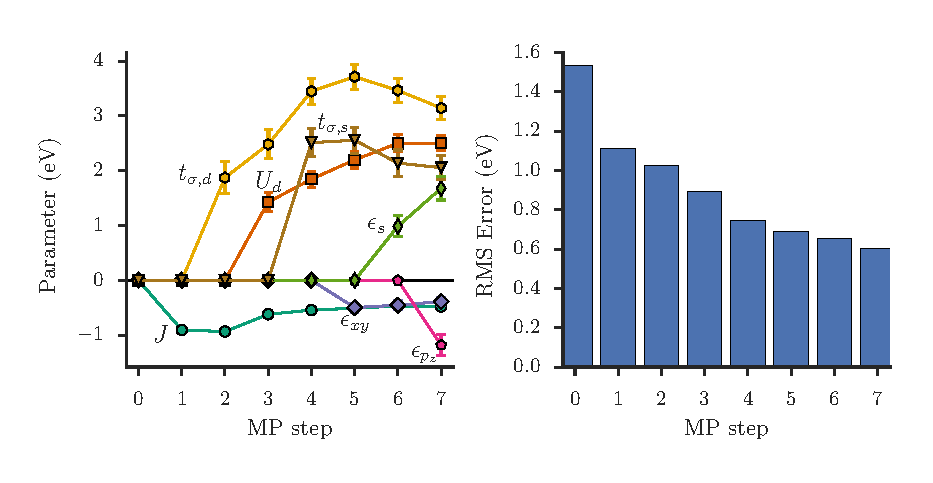
\includegraphics[width=0.8\textwidth]{./Figures/fese.eps}
  \caption{
    \label{fig:fese} 
    (Left) Parameter values for each fit generated in the MP algorithm, labeled at the step where they are included in the model. 
    A zero value indicates that parameter is not yet added to the model.
    The sign of $J$ is consistent with Hund's rules, and the signs of $t_{\sigma,d}$ and $t_{\sigma,s}$ are consistent with Se being located in positive $z$ with respect to Fe. 
    The $\epsilon_i$ states adjust the energies of the single particle orbitals relative to the energy of the other orbitals.
    (Right) RMS error of each model generated by MP as the algorithm includes parameters. 
  }
\end{figure*}

Applying the MP approach to the system produced reasonable parameter estimates, and suggested the Hund's coupling to be an important component of this model.
\lucas{too much passive, 'reasonable,' 'suggested'}
Figure~\ref{fig:fese}(a) and (b) show the evolution of the parameters and RMS error of the fit parameters are added one by one.
All previous parameters may change at each step because the entire model is refitted in each iteration.
The parameters are smoothly varying with the inclusion of new parameters, and their values are physically reasonable.
The matching pursuit algorithm would suggest that minimal models can be built by disregarding the descriptors added in later steps.
For this system, $J$ is considered the most important parameter\lucas{'most important' is vague. Don't use that construction.} in the model, and an absolute minimal model for the system would be $H_\text{minimal} = E_0 + J_d \sum_i S_i \cdot S_j$. 
Such a model would have an RMS error 1.11 eV. 
According to matching pursuit, the next most important interactions to include are (1) hopping between $d_{z^2}$ and $p_z$, (2) on-site $d$ Coulomb interactions, and (3) hopping between the $4s$ and the $p_z$, and so on. 
Including these degrees of freedom brings the RMS error to 0.75 eV.\lucas{What does this mean?} 
In this way, MP would suggest\lucas{MP doesn't suggest anything. Things don't suggest.}  that the most important interactions in the system at low energy are Hund's coupling, hopping between iron $3d$ and selenium $4p$, and on-site Coulomb repulsion, in that order.
This observation is consistent with the several studies in the literature, which find Hund's coupling in bulk FeSe to be an important part of its description~\cite{demedici_hunds_2011,de_medici_janus-faced_2011,georges_strong_2013,busemeyer_competing_2016}.

